\documentclass[10pt]{beamer} %[handout,red]
\usepackage{amsmath}
\usepackage{graphicx,multimedia,hyperref,xmpmulti}
\usepackage[utf8]{inputenc}
\usepackage[czech]{babel}

%%%%%%%%%%%%%%%%%%%%%%%%%%%%%%%%%%%%%%%%%%%%%%%%%%%%%%%%%%%%%%%%%%%%%%%%%%%%%%%%
% SYMBOLS
\def\div{{\rm div}}
\def\Lapl{\Delta}
\def\grad{\nabla}
\def\supp{{\rm supp}}
\def\dist{{\rm dist}}

\def\Tr{{\rm Tr}}
\def\sgn{{\rm sgn}}
\def\to{\rightarrow}
\def\weakto{\rightharpoonup}
\def\imbed{\hookrightarrow}
\def\cimbed{\subset\subset}
\def\range{{\mathcal R}}
\def\argdot{{\hspace{0.18em}\cdot\hspace{0.18em}}}
\def\Distr{{\mathcal D}}
\def\convol{\star}
\def\impl{\Rightarrow}
\DeclareMathOperator*{\esslim}{esslim}
\DeclareMathOperator*{\esssup}{ess\,sup}
\DeclareMathOperator{\ess}{ess}
\DeclareMathOperator{\osc}{osc}
\DeclareMathOperator{\curl}{curl}

% ****************************************** GENERAL MATH NOTATION
\def\Real{{\rm\bf R}}
\def\d{\,{\rm d}}               % differential

\def\vc#1{\mathbf{\boldsymbol{#1}}}     % vector
\def\tn#1{{\mathbb{#1}}}    % tensor
\def\abs#1{\lvert#1\rvert}
\def\Abs#1{\bigl\lvert#1\bigr\rvert}
\def\bigabs#1{\bigl\lvert#1\bigr\rvert}
\def\Bigabs#1{\Big\lvert#1\Big\rvert}
\def\ABS#1{\left\lvert#1\right\rvert}
\def\norm#1{\bigl\Vert#1\bigr\Vert} %norm
\def\close#1{\overline{#1}}
\def\inter#1{#1^\circ}
\def\ol#1{\overline{#1}}
\def\ul#1{\underline{#1}}
\def\eqdef{\mathrel{\mathop:}=}     % defining equivalence
\def\where{\,|\,}                    % "where" separator in set's defs
\def\timeD#1{\dot{\overline{{#1}}}}

% ******************************************* USEFULL MACROS
% enumerate by roman numbers
\def\RomanEnum{\renewcommand{\labelenumi}{\rm (\roman{enumi})}}   
% partial deriv.
\def\prtl{\partial} 
\def\Names#1{{\scshape #1}}
\def\rem#1{{\parskip=0cm\par!! {\sl\small #1} !!}}

\def\Xint#1{\mathchoice
{\XXint\displaystyle\textstyle{#1}}%
{\XXint\textstyle\scriptstyle{#1}}%
{\XXint\scriptstyle\scriptscriptstyle{#1}}%
{\XXint\scriptscriptstyle\scriptscriptstyle{#1}}%
\!\int}
\def\XXint#1#2#3{{\setbox0=\hbox{$#1{#2#3}{\int}$}
\vcenter{\hbox{$#2#3$}}\kern-.5\wd0}}
\def\ddashint{\Xint=}
\def\dashint{\Xint-}

% ******************************************* DOCUMENT NOTATIONS
% document specific
\def\rh{\varrho}
\def\th{\vartheta}
\def\dx{\,\d\vx}
\def\dt{\,\d t}
\def\eps{\varepsilon}
\def\phi{\varphi}
%%%%%%%%%%%%%%%%%%%%%%%%%%%%%%%%%%%%%%%%%%%%%%%%%%%%%%%%%%%%%%%%%%%%%%%%%%%%%%%%%%%%%


%%%%%%%%%%%%%%%%%%%%%%%%%%%%%%%%%%%%%%%%%%%%%%%%%%%%%%%%%%%%%%%%%%%%%%%%%%%%%%%%%
% Basic colors
%%%%%%%%%%%%%%%%%%%%
%\definecolor{background}{RGB}{238, 242, 249}       %grey
\definecolor{background}{RGB}{255,255,255}
% frame titles, section, enumrations, etc. (should match main color of logo)
%\definecolor{cxi}{RGB}{196,18,45}
\definecolor{cxi}{RGB}{225,114,21}
\definecolor{emph}{RGB}{196, 18, 45}
% complementary foregroung color, emphesize some text 
\definecolor{emph2}{RGB}{18, 4, 199}

\def\col{\textcolor}


% Templating stuff
% \beamertemplatetransparentcovereddynamic
%\colorlet{averagebackgroundcolor}{gray}
%\setbeamertemplate{itemize items}[circle]
%\setbeamertemplate{enumerate items}[square]
\setbeamertemplate{section in toc}[square]
%\setbeamercolor*{block title}{fg=white,bg=structure!75!black}
%\setbeamercolor*{block body}{bg=structure!10!averagebackgroundcolor}

%\setbeamercolor*{block title example}{fg=white,bg=beamerexample!75!black}
%\setbeamercolor*{block body example} 
%{bg=beamerexample!10!averagebackgroundcolor}
%\usepackage{beamerthemeshadow}
%\setbeamertemplate{background canvas}{\includegraphics 
%[width=0.3\paperwidth]{logo-cxi-cmyk-cz.pdf}}

\setbeamertemplate{footline}{
    
\includegraphics[width=\paperwidth]
    {graphics/fm-spojovaci.png}

    \vspace{-6mm}

    \hspace{5mm}{
        \bf\insertshorttitle~ \textcolor{structure}{$\boldsymbol{|}$} 
        \insertdate
    }

    \vspace{-3.1mm}

    \hspace{\stretch{1}} 
    \textcolor{white}{\insertframenumber/\inserttotalframenumber} \hspace{2mm}

    \vspace{3mm}
}


\setbeamercolor{structure}{fg=cxi, bg=background}
\setbeamertemplate{frametitle}
{
    \begin{flushleft} 
        \bf\large\insertframetitle
    \end{flushleft}
    \par
}

\beamertemplateheadempty
\beamertemplatenavigationsymbolsempty
\beamertemplateshadowblocks



%\AtBeginSection[]
%{
%\frame{\frametitle{Obsah}
%  \tableofcontents[currentsection]
%}
%\addtocounter{framenumber}{-1} 
%}

%***************************************************************************

%%%%%%%%%%%%%%%%%%%%%%%%%%%%%%%%%%%%%%%%%%%%%%%%%%%%%%%%%%%%%%%%%%%%%%%%%%%%%%%%
%%%%%%%%%%%%%%%%%%%%%%%%%5

%\AtBeginSection[]
%{
% \begin{frame}<beamer>
% \frametitle{Plan}
% \tableofcontents[currentsection]
% \end{frame}
%}



\title[Fast non-matching grids]{
\textcolor{emph2}{Fast intersections of non-matching grids\\ using the Pl\"ucker coordinates.}
\vspace{2ex}
}

\author{{\bf Jan Březina}, Pavel Exner, Jan Stebel}
\institute{Technical University of Liberec, Czech Rep.}
\date{ESCO, June 2016}





\begin{document}
%\setbeamercolor{background canvas}{bg=gray}


{  
    \setbeamercolor{background canvas}{bg=background} 
    \setbeamertemplate{background}
    {
        
        %
\includegraphics[width=0.5\paperwidth]{graphics/logo-cxi-cmyk-en.pdf}
        
\includegraphics[width=0.5\paperwidth]{graphics/logo-fm-cmyk-en.pdf}

    }
    
    \setbeamertemplate{footline}
    {
\includegraphics[width=\paperwidth]{graphics/fm-spojovaci.png}
        
        \vspace{-6mm}
        \hspace{5mm}
        {\bf TECHNICAL UNIVERSITY OF LIBEREC 
            \textcolor{structure}
            {$\boldsymbol{|}$ Fakulty of mechatronics}
        }
        \textcolor{structure}{$\boldsymbol{|}$} fm.tul.cz

        \vspace{-3.1mm}
        \hspace{\stretch{1}} 
        \textcolor{white}{\insertframenumber/\inserttotalframenumber} 
        \hspace{2mm}

        \vspace{3mm}
    }
    
    \begin{frame}    
        \vspace{1cm}
        {\bf\large\inserttitle}\\
        \vspace{2mm}
        \textit{\insertauthor~ \textcolor{structure}{$\boldsymbol{|}$} \insertdate}
    \end{frame}
}


\begin{frame}{Primary motivation: Geometry with multiscale features}
    \noindent
    \hbox{
    \begin{minipage}{0.5\linewidth}
        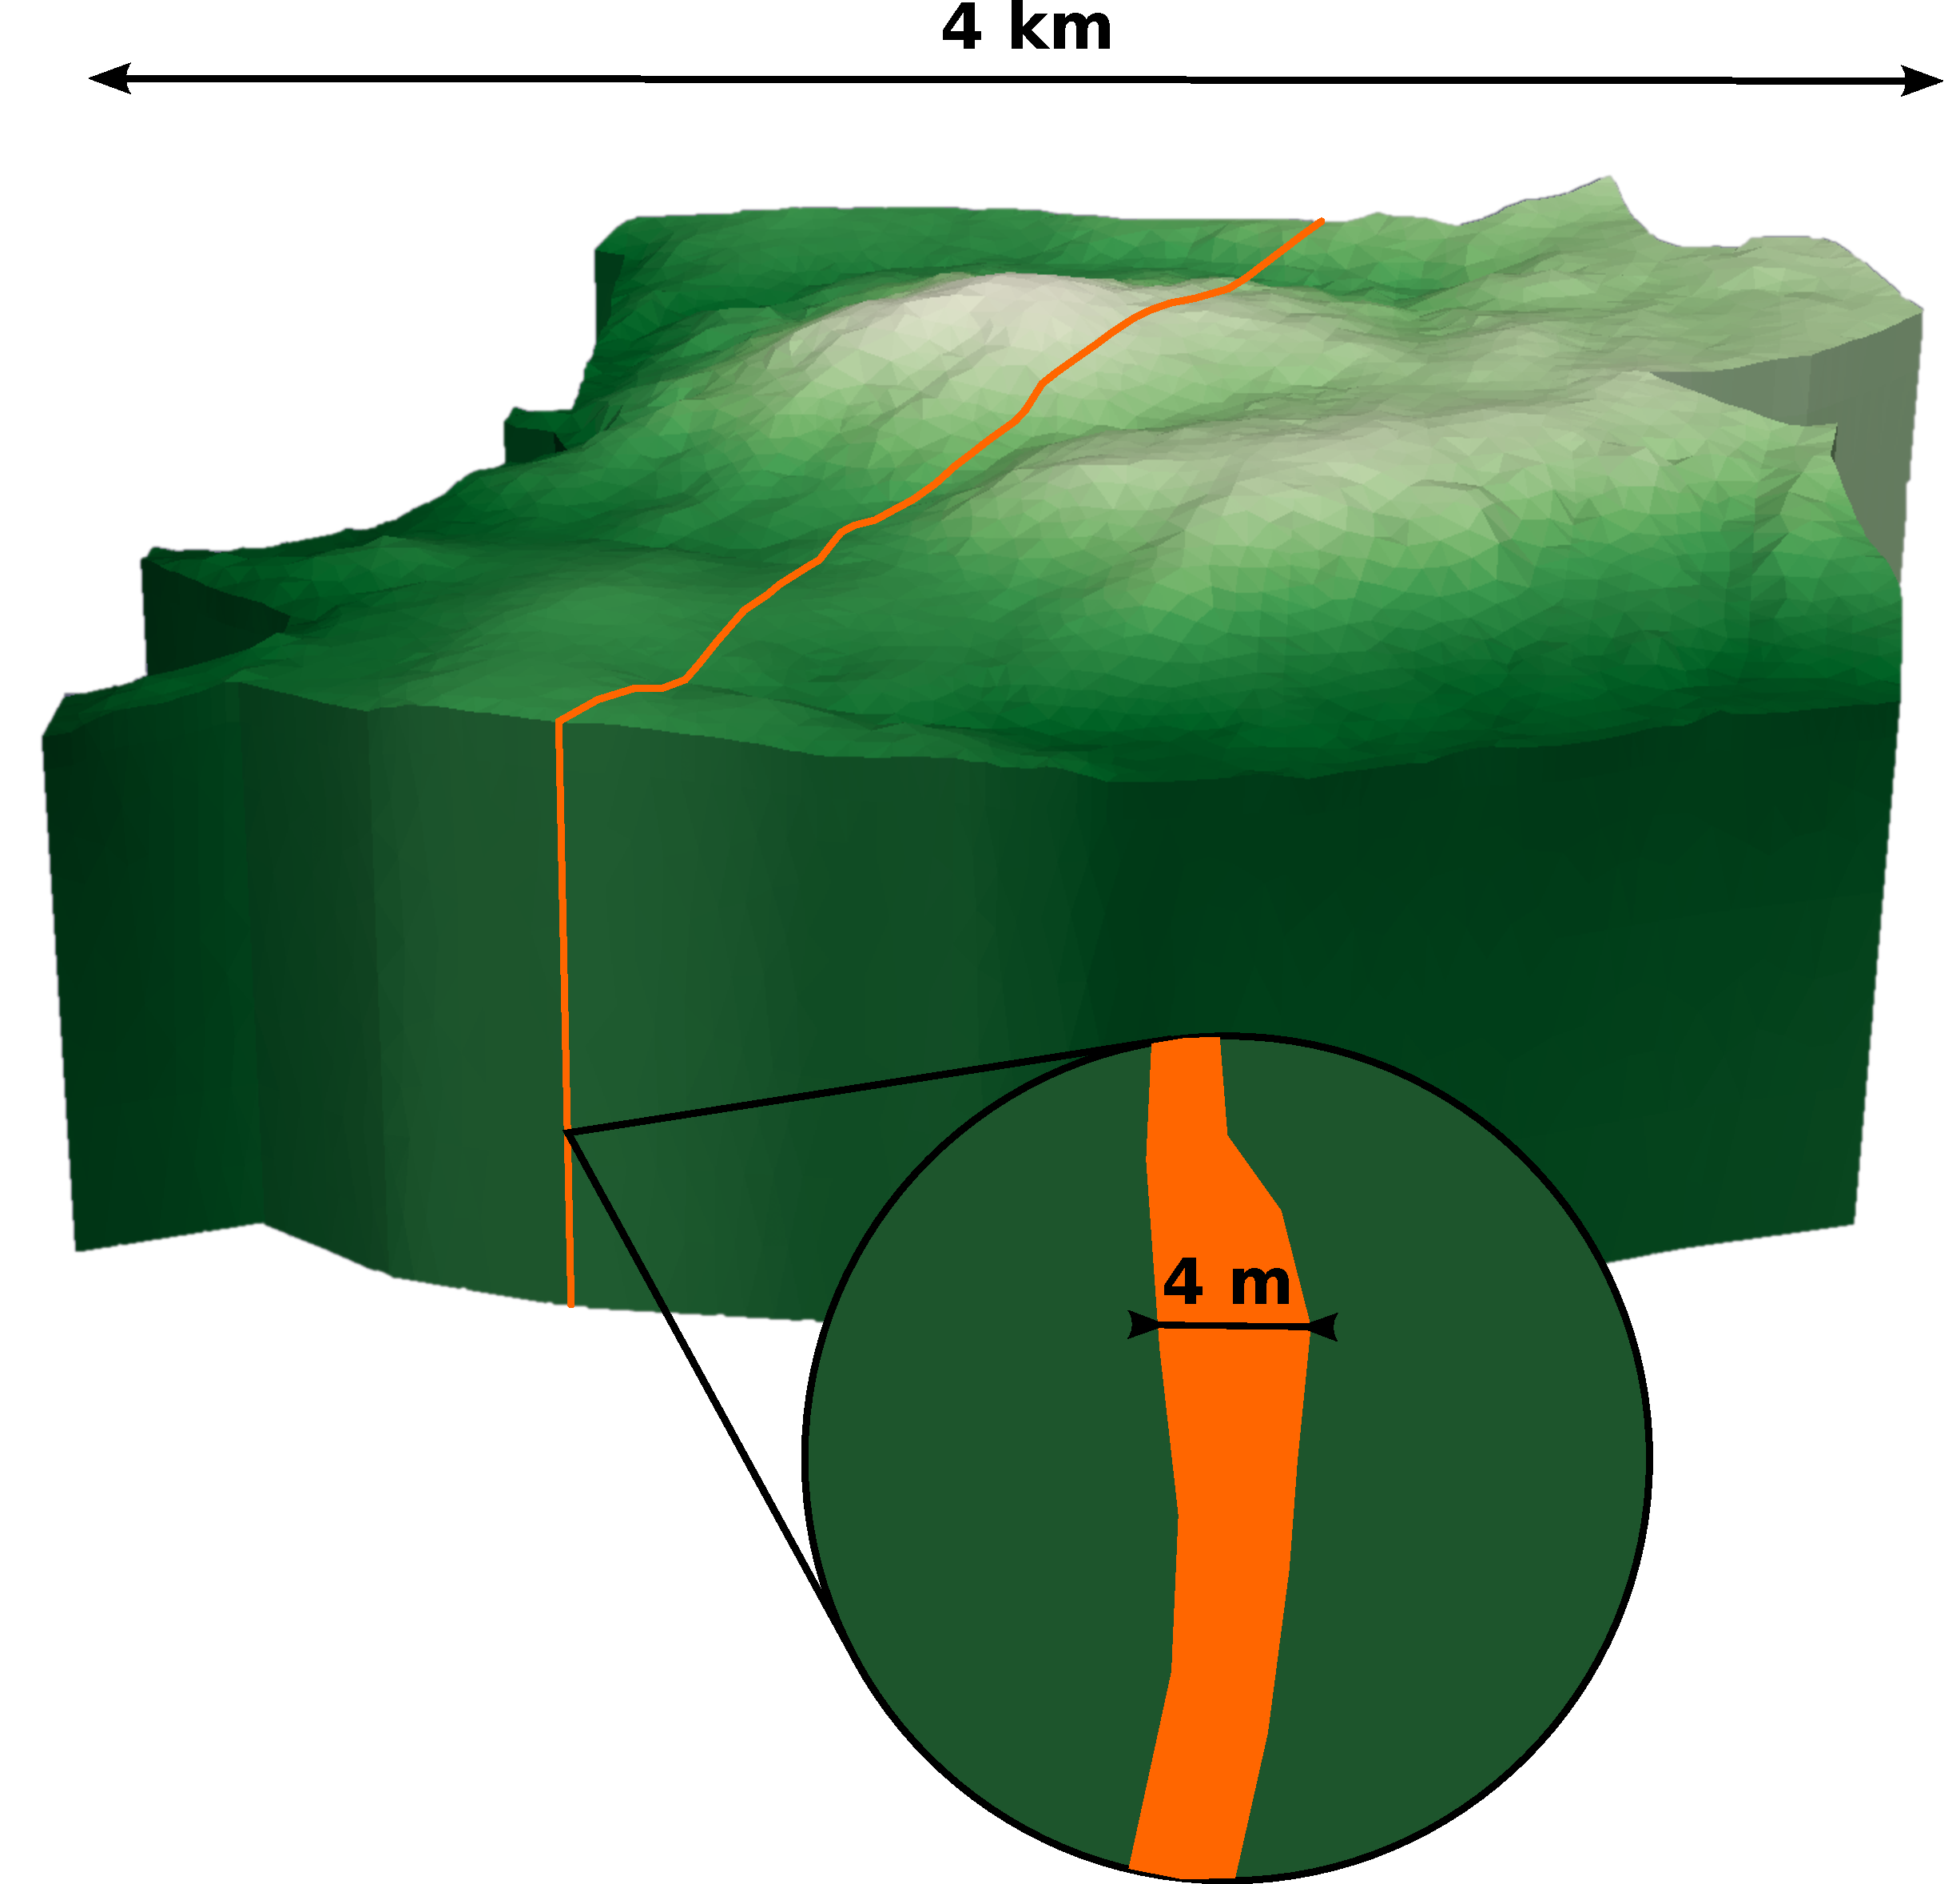
\includegraphics[width=\linewidth]{graphics/melechov_scale.pdf}
    \end{minipage}
    \begin{minipage}{0.5\linewidth}
        \begin{itemize}
        \item Candidate locality for a nuclear waste deposit in the Czech Republic.
        \item Plutonic rock with significant fracture zones.
        \item Fracture zones: Small flux, big velocity $\impl$
        \item Possible fast transport of polutants (preferential paths).
        \end{itemize}
        
        \vspace{2ex}
        \begin{itemize}
        \item Large, but thin fracture zones leads
              to a multiscale problem.
        \item Direct discretization is impractical.
        \item Our approach: fractures as lower dimensional objects.
        \end{itemize}
    \end{minipage}
    }
\end{frame}

\begin{frame}{Integrating accross the fracture}
    \begin{minipage}{0.40\textwidth}
    Coupled 2D domains accross boundary.
    \begin{center}
        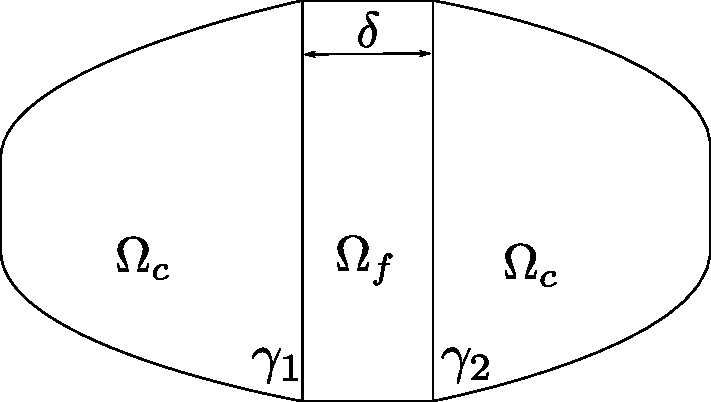
\includegraphics[width=\linewidth]{graphics/continuum_model_domain.pdf}
    \end{center}    
    \end{minipage}
    \hspace{1ex}$\longrightarrow$\hspace{1ex}
    \begin{minipage}{0.40\textwidth}
        Coupled 2D continuum with the fracture 1D model.
        \begin{center}
                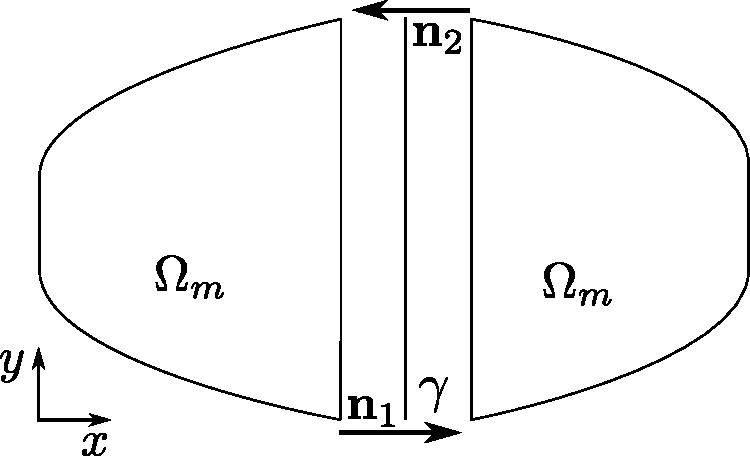
\includegraphics[width=\linewidth]{graphics/fracture_model_domain.pdf}
        \end{center}
    \end{minipage}
    
    \vspace{2ex}
    \textcolor{blue}{Related works:}\\
    {\small
    {\bf Martin, Jaffr{\'e}, Roberts} : {\it Modeling Fractures and Barriers ...}, 2005

    \vspace{1ex}
    {\bf Angot, Boyer, Hubert} : {\it Asymptotic and numerical modelling ...}, 2009
    
    \vspace{1ex}
    {\bf B., Stebel} :  {\it Analysis of Model Error ...}, 2015
    }    
\end{frame}



\begin{frame}{Why we need non-matching grids?}
\begin{center}
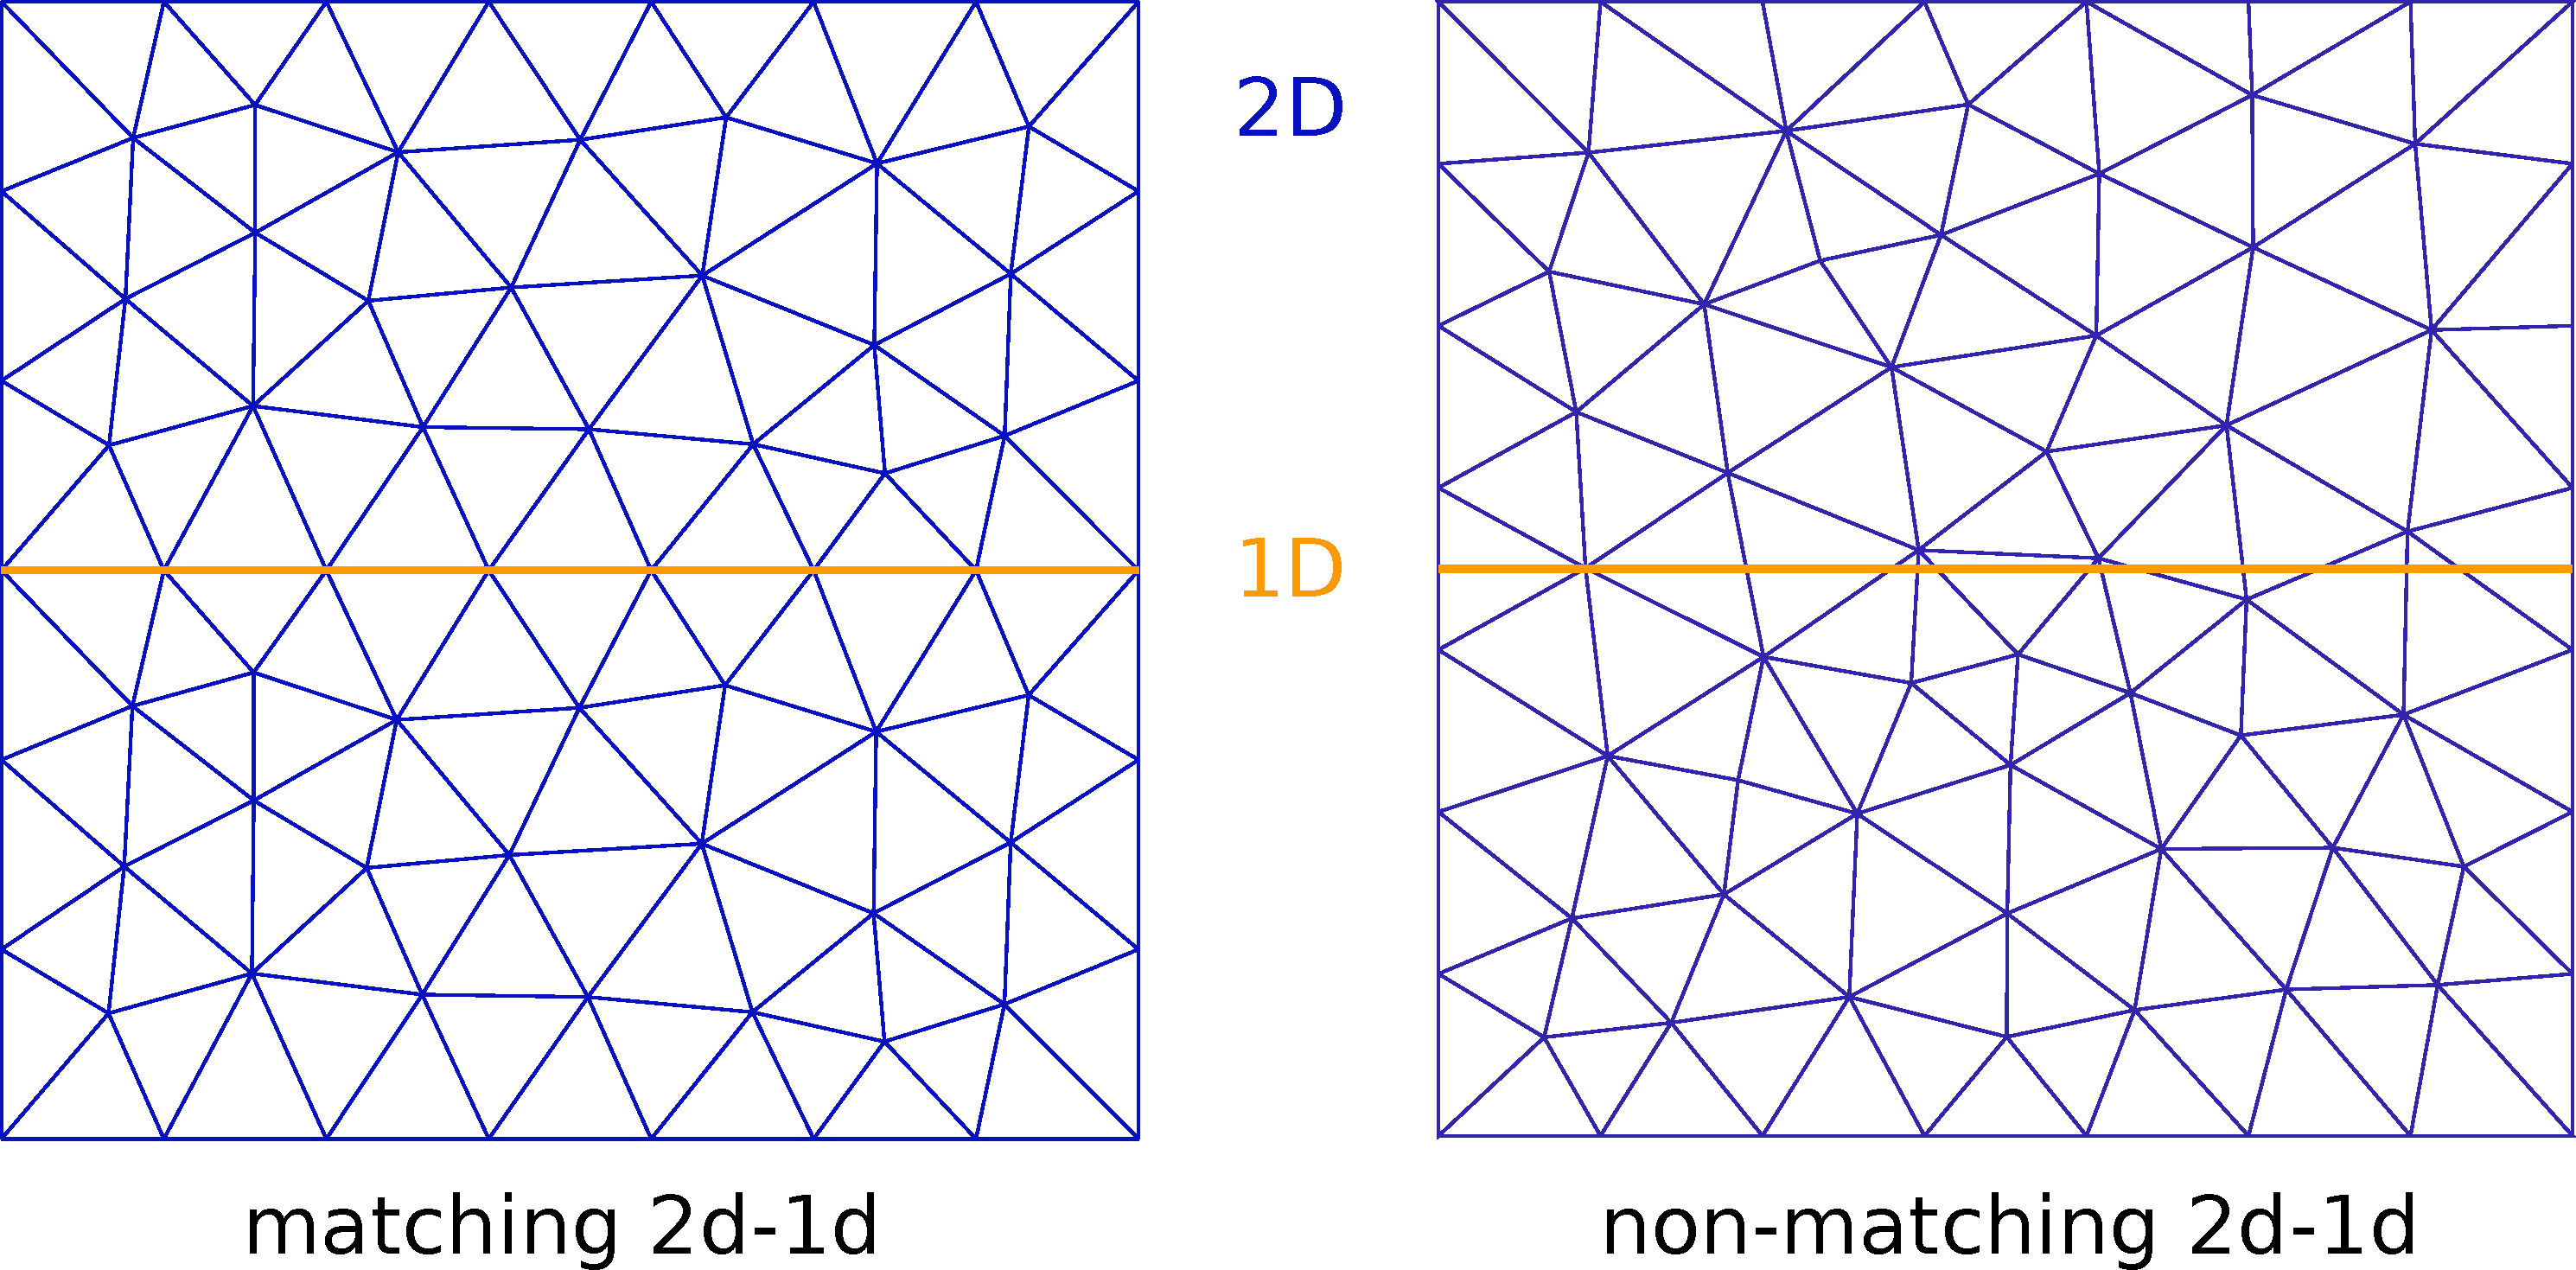
\includegraphics[width=0.6\linewidth]{graphics/compatible_noncompatible.pdf} 
\end{center}

\begin{itemize}
 \item resolve dificulties with complex geometry (thousends of fractures)
 \item simplify mesh generation
 \item allow changing geometry (e.g. crack propagation)
 \item possible usage in a multi mesh approach
\end{itemize}

\end{frame}


\begin{frame}{What we need?}
\begin{itemize}
  \item universal algorithm(s): 3D-2D, 2D-1D, 3D-1D, 2D-2D  
  \item fast algorithm: milions of elements, dense fracture networks
  \item robust algorithm, e.g. 
\end{itemize}

\vspace{2ex}
All intersections based on line-triangle intersections.\\

\vspace{2ex}
Inspiration by computer graphics algorithms, ray-triangle.\\
Pl\"ucker coord. apprach. (Platis, Theoharis, 2003) 
\end{frame}


\begin{frame}{Pl\"ucker coordinates}
  The line $p$, direction vector $\vc u$ going through the point $\vc A$.\\
  \textcolor{blue}{Pl\"ucker coordinate:}
  \[
    \pi_p = (\vc u_p, \vc v_q) =( \vc u, \vc u \times \vc A).
  \]
  
  \vspace{2ex}
  \textcolor{blue}{Scalar product:}
  \[
     \pi_p \cdot \pi_q = \vc U_p \cdot \vc V_q + \vc U_q \cdot \vc V_p,
  \] 
  
  \vspace{2ex}
  
  \begin{center}
  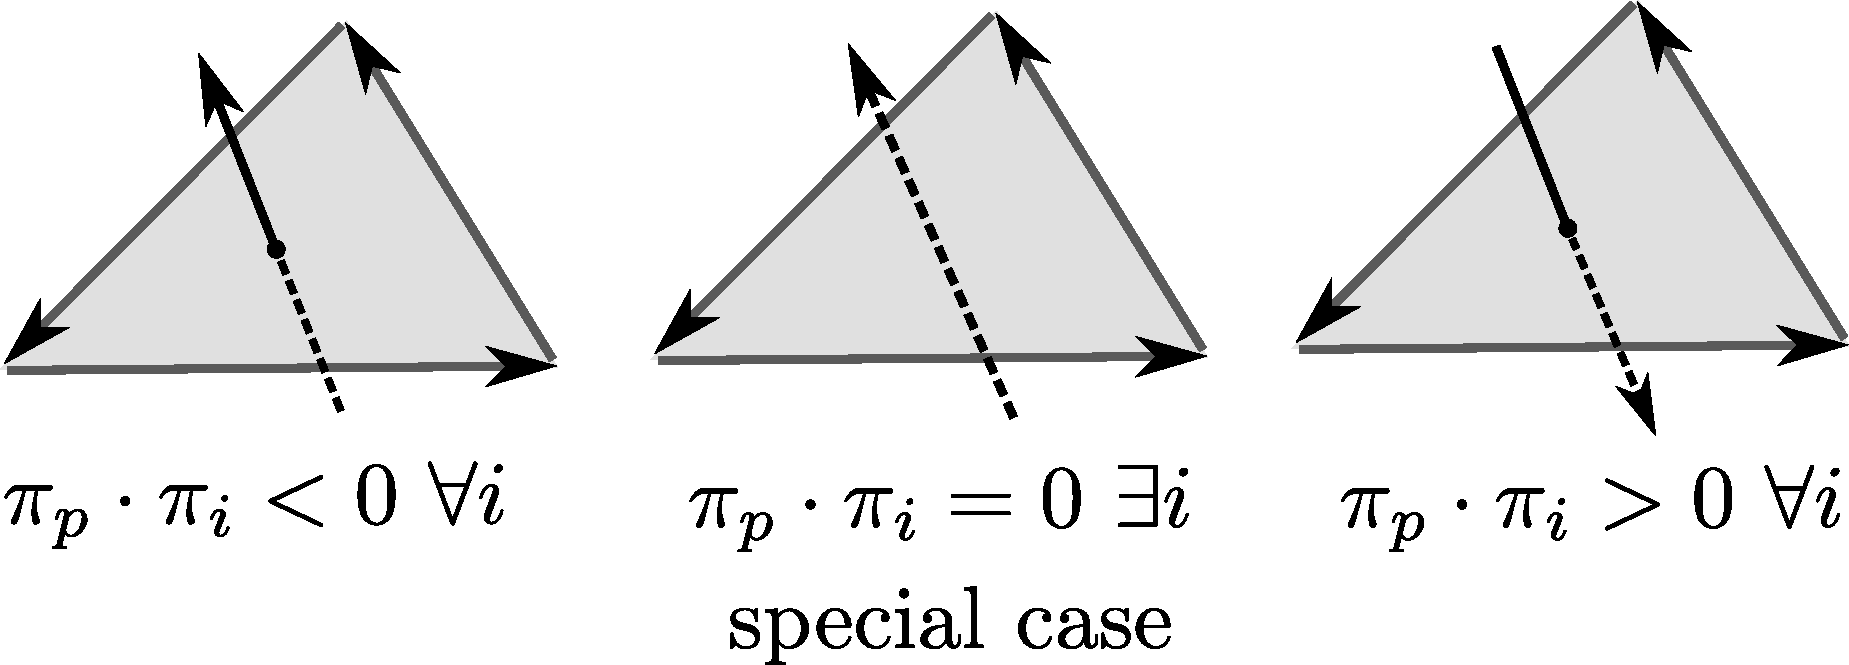
\includegraphics[scale=0.2]{graphics/plucker_product.pdf} 
  \end{center}
\end{frame}

\begin{frame}{Barycentric coordinates}
    \textcolor{blue}{On triangle:}
        \[
        x_i = \frac{\pi_p \cdot \pi_i}{\sum_{j=1}^{3} \pi_p \cdot \pi_j}
        \]
    \textcolor{blue}{On line $\vc A + t\vc U$:}
        \[
        y_0 = \frac{\abs{\vc X - \vc A}}{\abs{\vc U}}
        \] 
    \textcolor{blue}{On tetrahedra:}
        Append one zero coordinate (depending on the face).
\end{frame}


\begin{frame}{Intersection polygon (2D-3D)}
\begin{itemize}
 \item Need to sort intersections to form convex polygon.
 \item Standard convex hull algorithms ... slow, further float operations.
 \item Reusing signs of Pl\"ucker products, we get correct order ...
\end{itemize}
\end{frame}

\begin{frame}{Intersection polygon (2D-3D)}
    \begin{itemize}
     \item Polygon sides formed by triangle sides (S), tetrahedra faces (F).
     \item Intersection point connect particualar S with particular F.
     \item Order is given by triangle side orientation (SS, SF) or P\"ucker sign (FF).
    \end{itemize}
    \begin{center}
    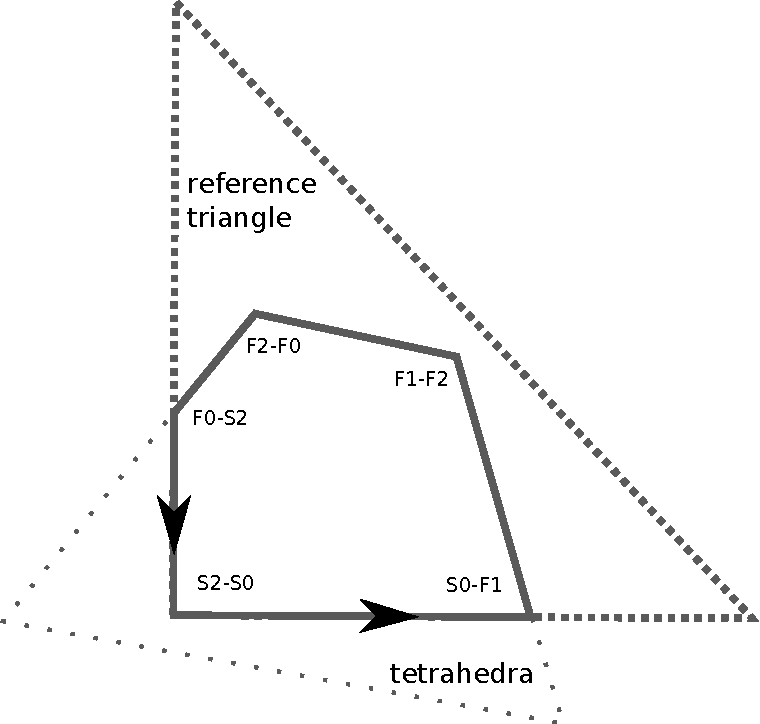
\includegraphics[scale=0.4]{graphics/polygon_tracing.pdf} 
    \end{center}   
\end{frame}

\begin{frame}{Efficiency (2D-3D)}
    \begin{minipage}{0.45\textwidth}
        \begin{tabular}{l|l}
            algorithm, 2D-3D& FLOPs\\
                      & estimate\\
            \hline\\
            parametric plane & 585\\
            normal plane (reuse) & 765\\
            Moller and Trumbore & 783\\
            Pl\"ucker (reuse) & 306
        \end{tabular}
        \vspace{4em}
    \end{minipage}
    \hspace{2ex}
    \begin{minipage}{0.45\textwidth}
        \begin{center}
            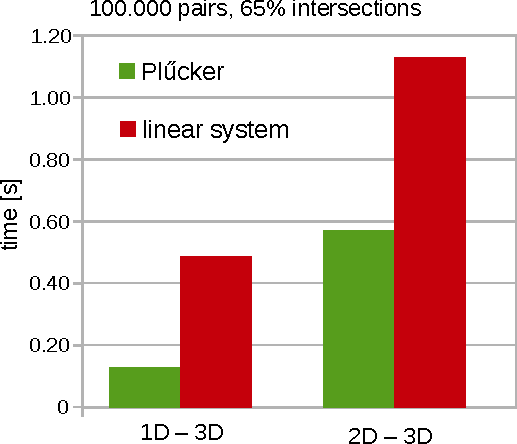
\includegraphics[width=1.2\textwidth]{graphics/intersections_fundamental_speed.pdf}
        \end{center}

    \end{minipage}
\end{frame}

\begin{frame}{Intersection of meshes}
  breath first search, algorithm 2D-3D, 1D-3D:
  \begin{enumerate}
    \item Get next unprocessed 2D element $k$.
    \item Find intersection candidates $\mathcal K$ in 3D mesh.
    \item For $K\in \mathcal K$ check intersection $(k, K)$.  
    \item Push the intersection neigbours into queues: $(k, L) \to Q_3$, $(l, K) \to Q_2$. 
    \item While $(l, L) \in Q_3$ check intersection $(l, L)$. Append queues.
    \item Pop pair from $Q_2$. (move to the next 2D element)
  \end{enumerate}

  \vspace{2ex}
  Issues:
  \begin{itemize}
   \item Need information about element connectivity (preprocessing).
   \item Mark and check already inspected pairs. Marking elements + hashing.
   \item Find the starting intersection. Use AABB (axes aligned bounding boxes) possibly with Bounding Interval Hierarchy. 
   \item Pass already known information with pairs.
   \item Deal with degenerated cases.
  \end{itemize}
\end{frame}

\begin{frame}{Scaling on artificial mesh}
  Cube with two diagonal fractures.
  
  \vspace{3ex}
  \hspace{-5ex}  
  \begin{minipage}{0.55\textwidth}
    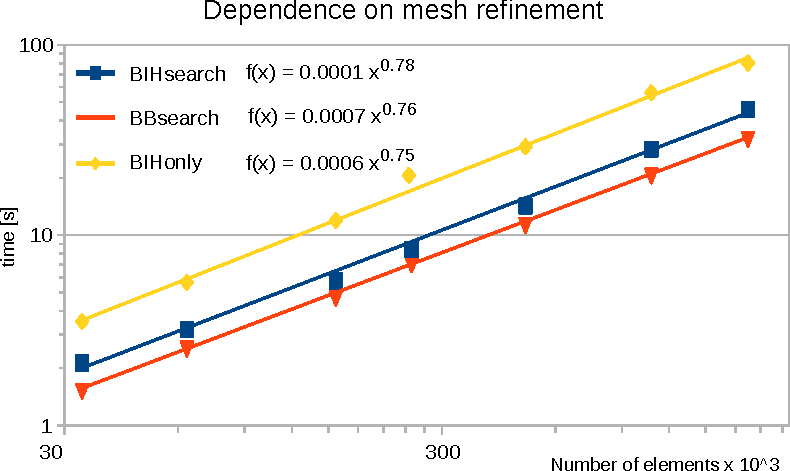
\includegraphics[scale=0.5]{graphics/intersections_test1_cube_speed_scaling.pdf}
    %\vspace{4em}
  \end{minipage}
  \hspace{5ex}
    \begin{minipage}{0.4\textwidth}
    \begin{center}
    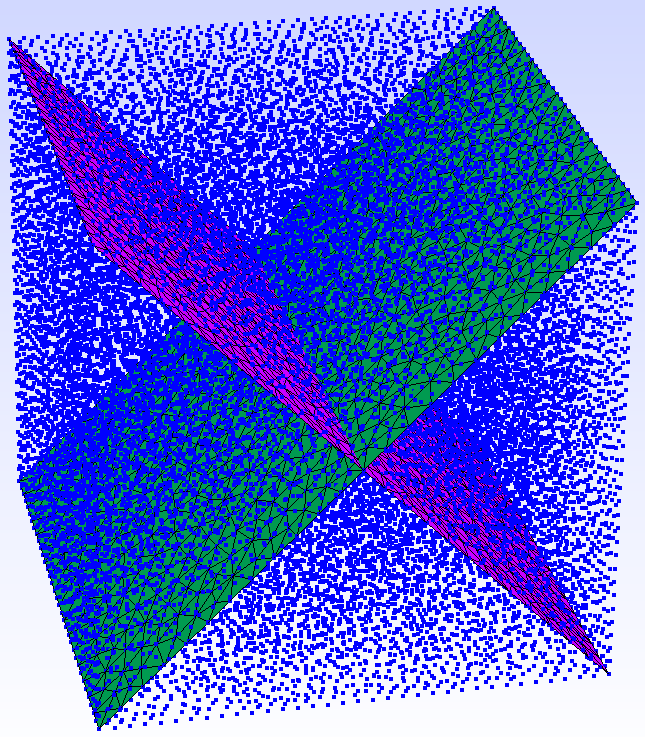
\includegraphics[scale=0.2]{graphics/cube_mesh.png} 
    \end{center}
    \end{minipage}
\end{frame}


\begin{frame}{Performance on a real world problem}  
    
    \begin{center}
    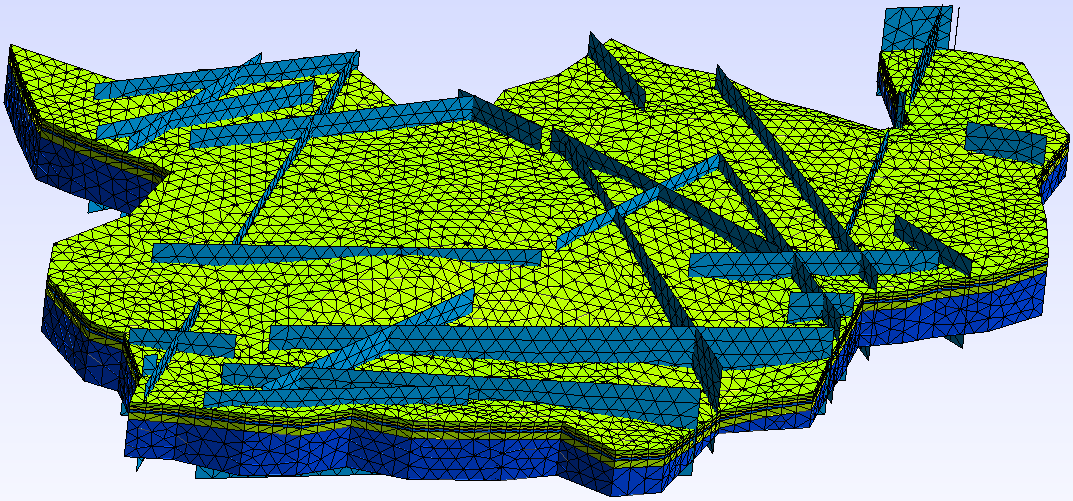
\includegraphics[scale=0.25]{graphics/bedrichov_mesh.png}
    \end{center}    
    
    \begin{center}
    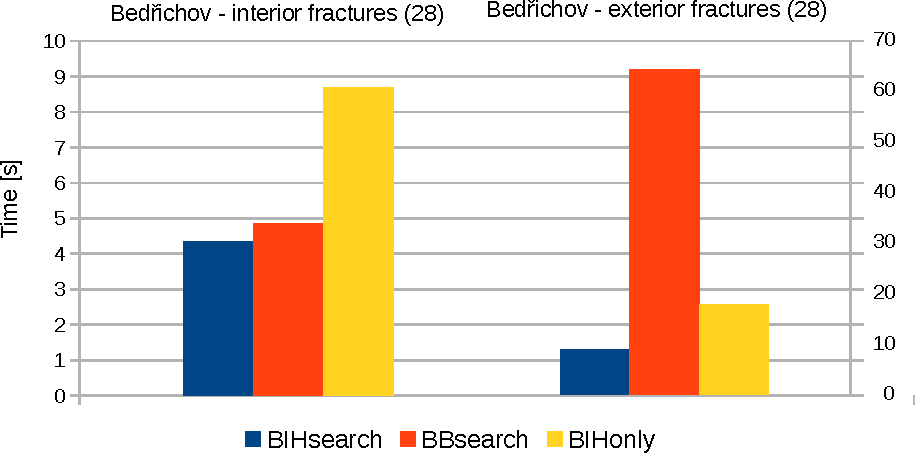
\includegraphics[scale=0.55]{graphics/intersections_bedrichov_both_speed.pdf}     
    \end{center}    
\end{frame}


\begin{frame}{Flow123d : \textcolor{black}{\bf flow123d.github.com}}
    \hbox{
        \hspace{6ex}
        \begin{minipage}{\linewidth}
            \includegraphics[scale=0.35]{graphics/real_appl.pdf}
        \end{minipage}
        \hspace{-1.15\linewidth}
        \begin{minipage}{\linewidth}
            
            \vspace{10ex}
            \begin{itemize}
             \item Software for hydrogeological modeling.
             \item \textcolor{blue}{Models on combination of 3d, 2d, 1d} simplicial elements
             \item Open source, C++
            \end{itemize}
        \end{minipage}
    }
\end{frame}


\begin{frame}{Flow123d - models}
\parindent 4ex

\noindent
\textcolor{emph2}{Darcy Flow}\\
steady and unsteady problems,\\
Lumped Mixed-Hybrid method, $RT_0$ elements\\ 

\vspace{2ex}
\noindent
\textcolor{emph2}{Solute Transport}\\
explicit FV, pure convection,\\
implicit Discontinuous Galerkin (arbitrary order), diffusion-dispersion

\vspace{2ex}
\noindent
\textcolor{emph2}{Reaction Term}\\
operator splitting\\
equilibrium sorption (fast interpolation algorithm)\\
dual porosity\\
decays, linear reactions

\vspace{2ex}
\noindent
\textcolor{emph2}{Heat transfer}\\
liquid-solid thermal equilibrium,\\
implicit Discontinuous Galerkin

\end{frame}

\begin{frame}{Application of non-matching meshes}
 ... work in progress: ...
\end{frame}

\begin{frame}{Darcy flow, 2D-1D interaction}
    
 \begin{center}
  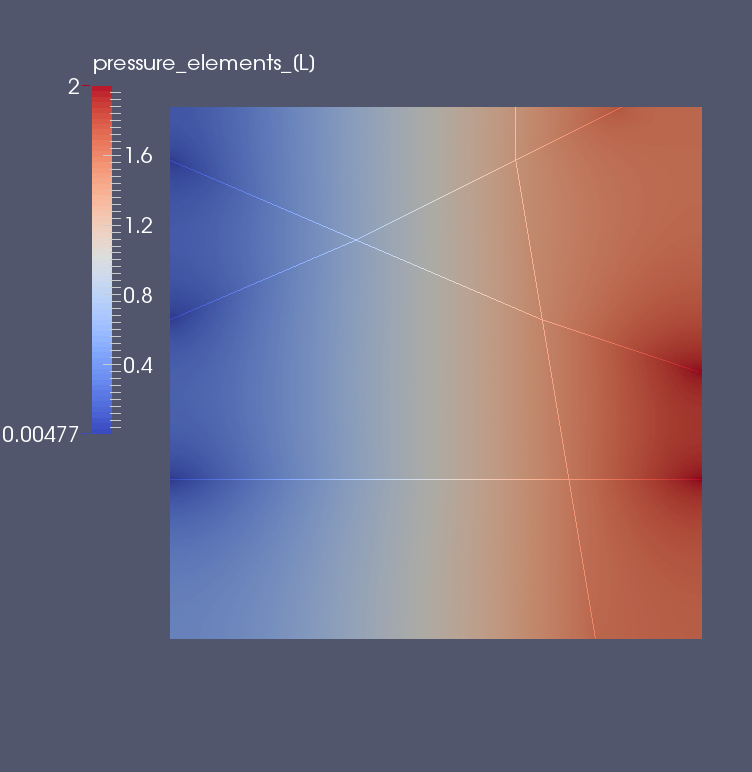
\includegraphics[scale=0.2]{graphics/boundary_P1.png}
   % boundary_P1.png: 752x772 pixel, 72dpi, 26.53x27.23 cm, bb=0 0 752 772
  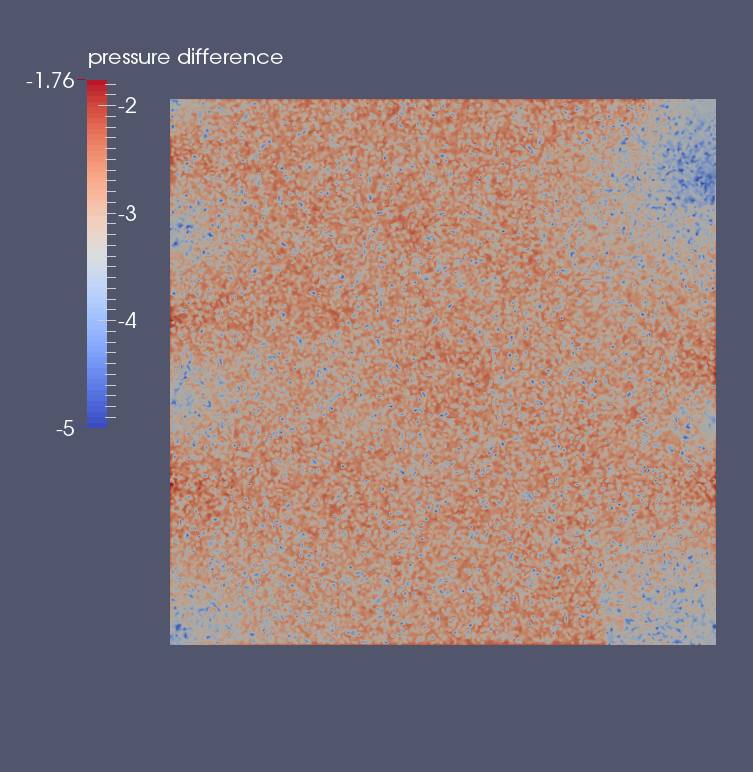
\includegraphics[scale=0.2]{graphics/boundary_P1-comp.png}
   % boundary_P1-comp.png: 753x772 pixel, 72dpi, 26.56x27.23 cm, bb=0 0 753 772
 \end{center}

 {\bf Left: } Pressure head computed by P1 method,\\
              domain $[-1,1] \times [-1,1]$.
 
 {\bf Right: } Difference between non-compatible P1 coupling \\
 and compatible coupling, log scale, $h=0.01$

\end{frame}

\begin{frame}{Wells: 3D-1D, XFEM}
    Goal: capture log cone aroung wells without increasing n. of DOFs
     \vspace{2ex}
     \begin{minipage}{0.4\linewidth}
         \centering
         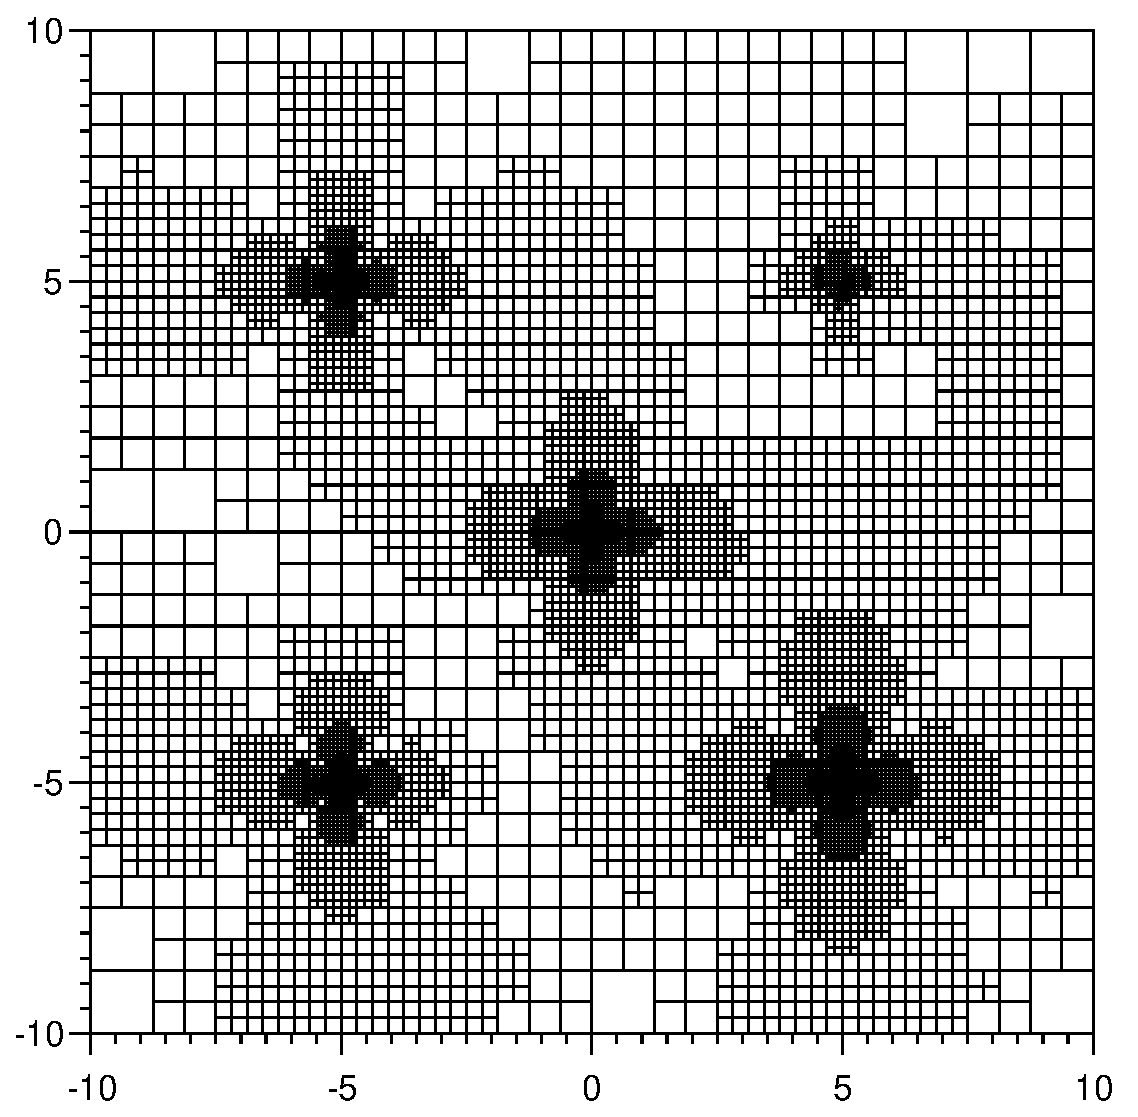
\includegraphics[width=0.8\linewidth]{graphics/five_wells_mesh1.pdf}
         
         \centering
         {\footnotesize adaptive FEM, mesh,\\ 30k elements, 171s}
     \end{minipage}
     \hspace{3em}
     \begin{minipage}{0.4\linewidth}
         \centering
         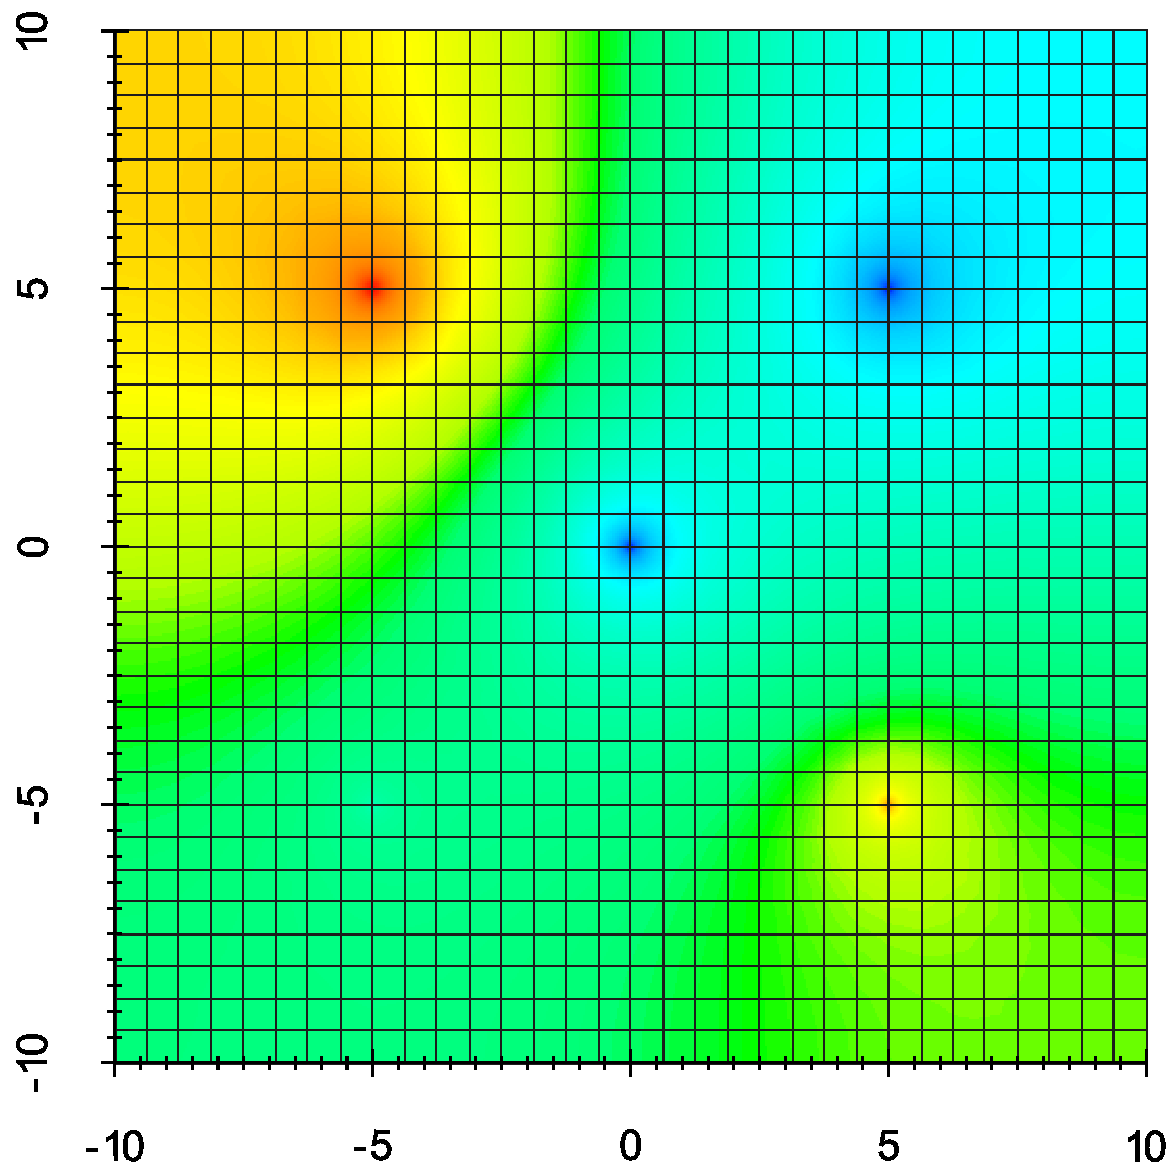
\includegraphics[width=0.8\linewidth]{graphics/five_wells_mesh2.pdf}
         
         \centering            
         {\footnotesize XFEM mesh and solution,\\ 1k elements, 17s}
     \end{minipage}

 Key ingredients:
 \begin{itemize}
    \item Find intersections.
    \item Suitable enrichment (for the mixed method).
    \item Adaptive integration in assembly.
  \end{itemize}  
  \vspace{-1ex}
  \hfill\hbox{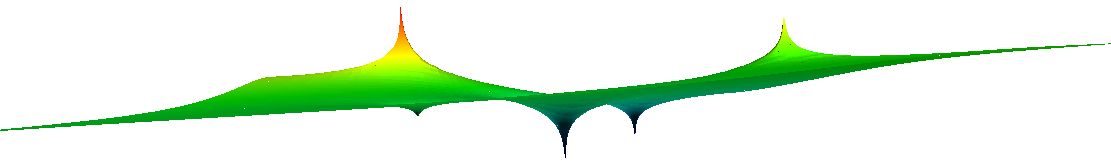
\includegraphics[width=0.7\linewidth]{graphics/warp_five_wells_alpha.png}}
\end{frame}

\begin{frame}{Elasticity of composits: 3D-1D}
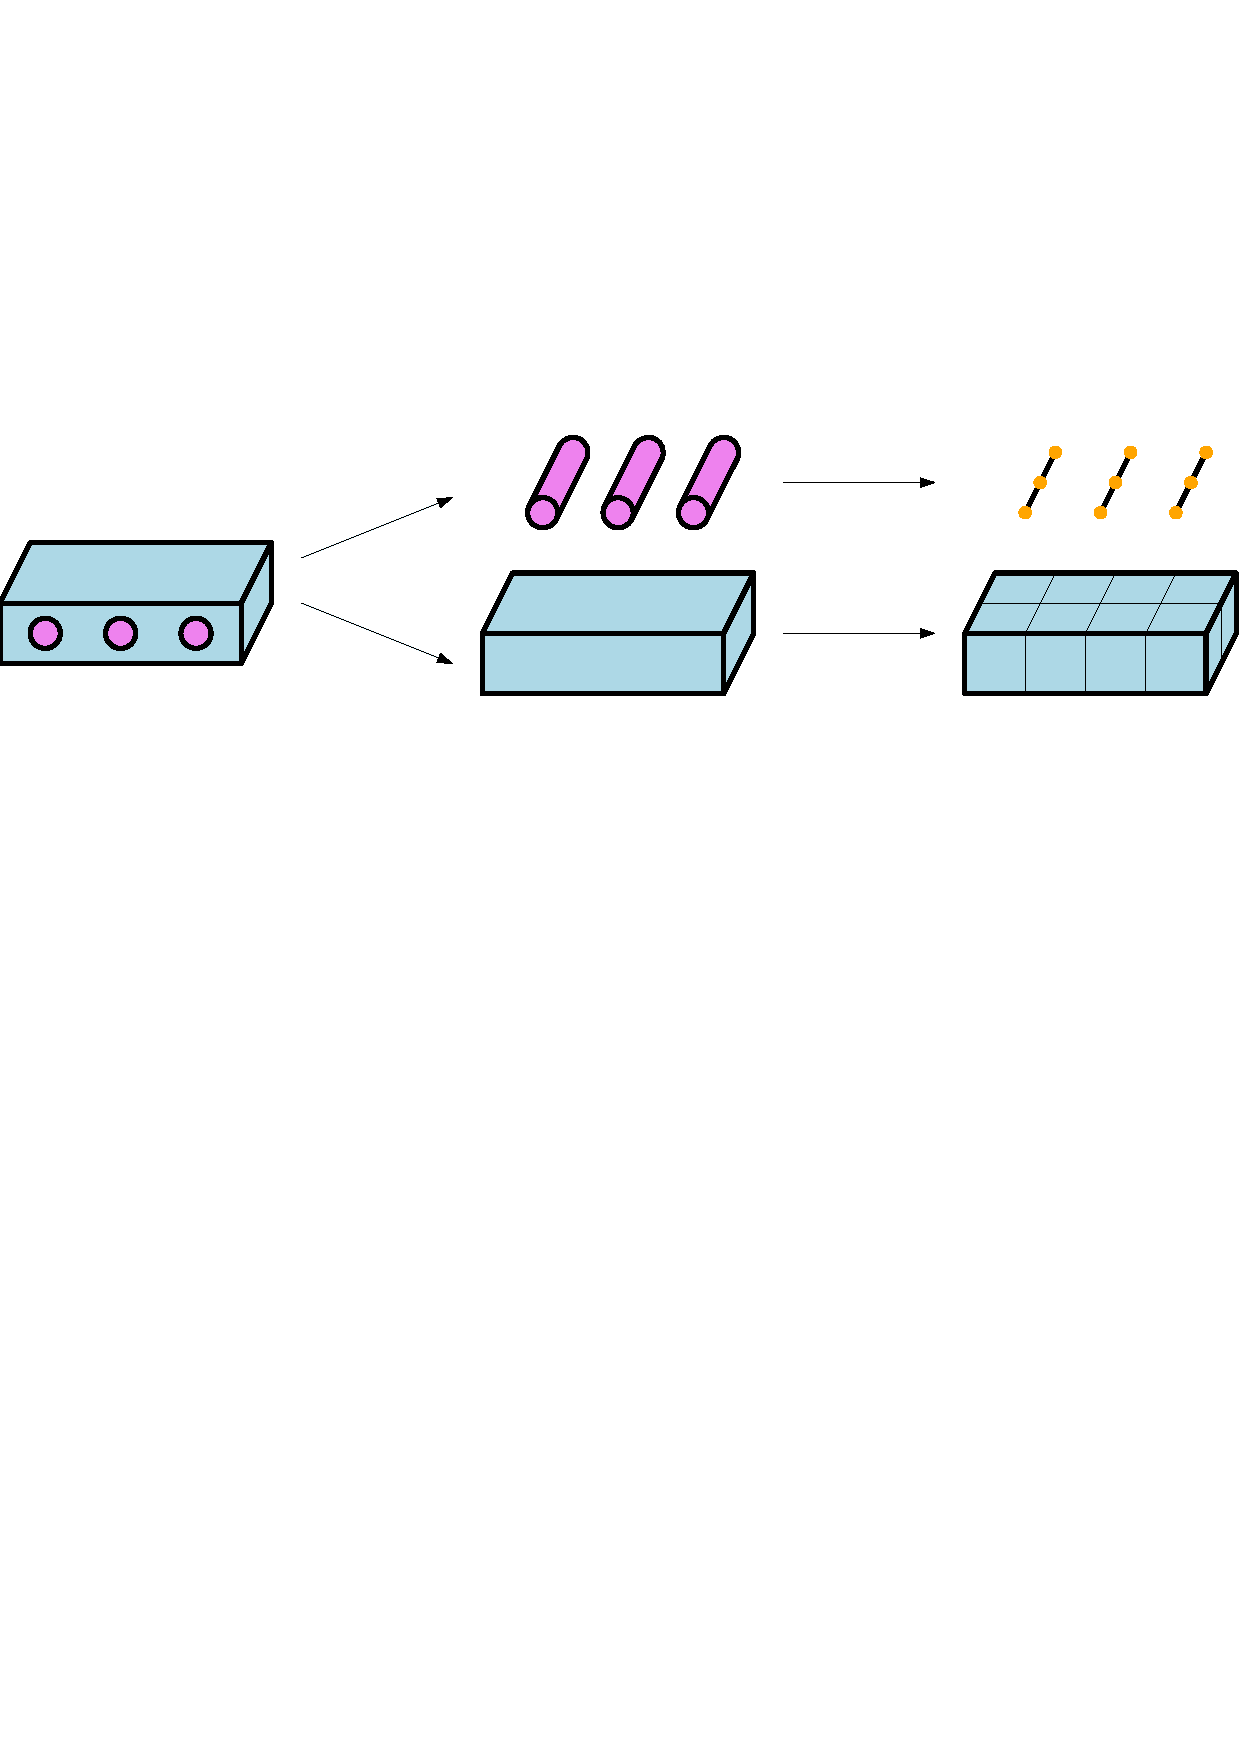
\includegraphics[width=10cm]{graphics-js/matrix-fibers}
\begin{itemize}
\item 3D structure with filament enforcement (polymer composites, stents)
\item 3D-1D non-matching grids, XFEM approach
\end{itemize}

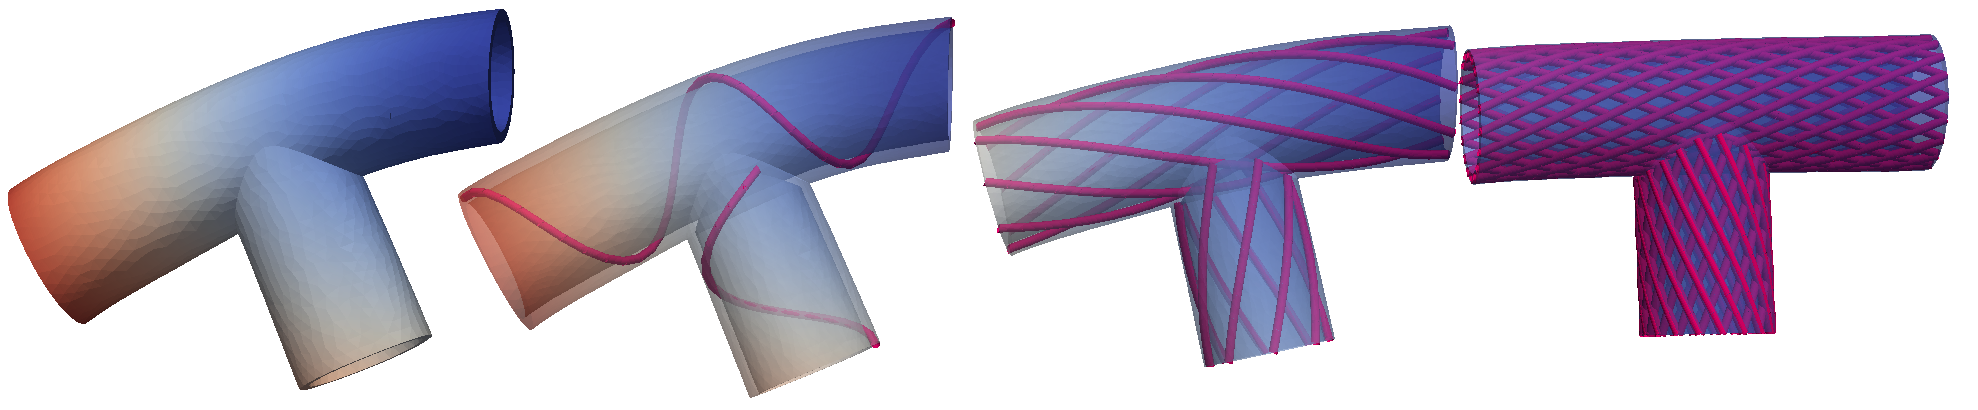
\includegraphics[width=10cm]{graphics-js/T-bend}

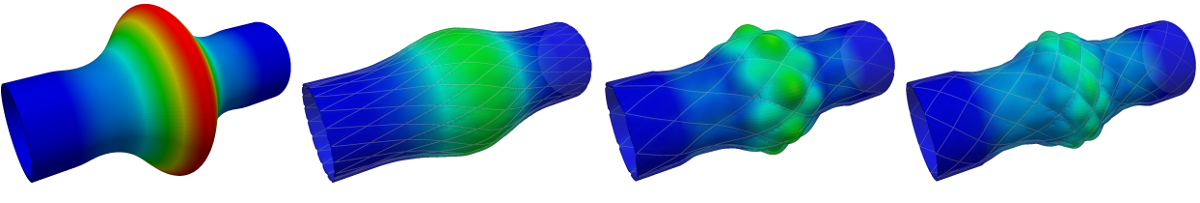
\includegraphics[width=10cm]{graphics-js/pipes}
\end{frame}

\begin{frame}{Changing geometry: vocal cord simulation}
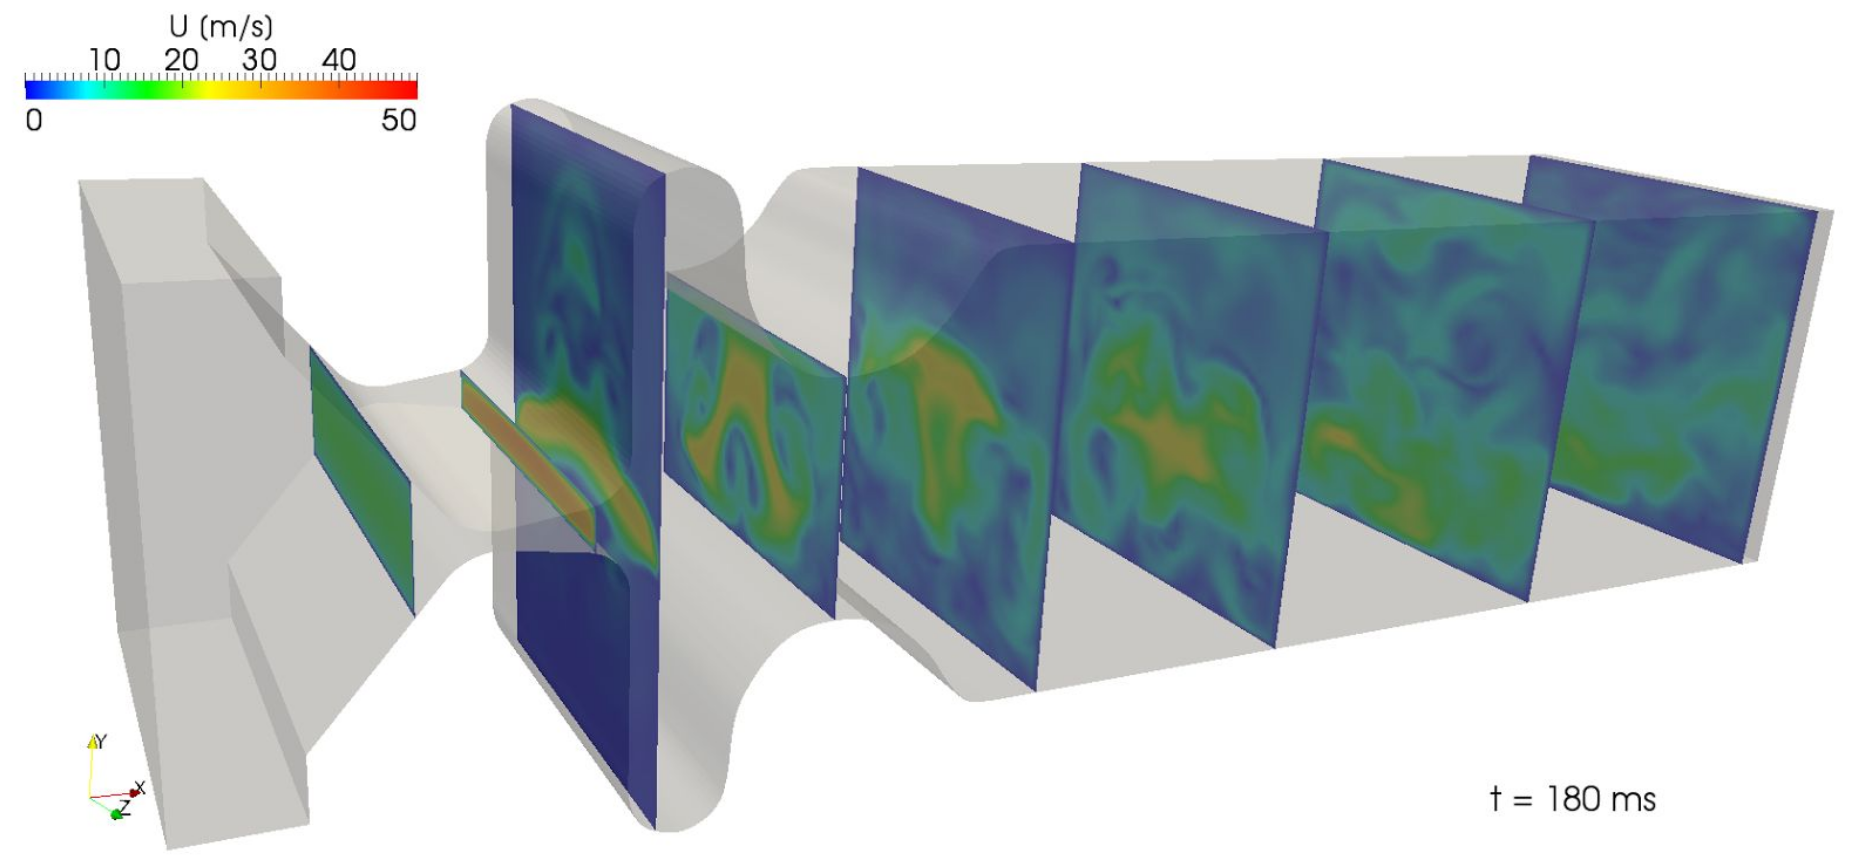
\includegraphics[width=10cm]{graphics/vocal_tract.png}

\begin{itemize}
 \item problem with contact - change in topology
 \item possible use of Immersed Boundary Method, need 3D-2D intersections
\end{itemize}
\end{frame}


\begin{frame}{Summary}
\begin{itemize}
 \item Mixed dimesion grids and models as solution of some multisclae problems.
 \item Mesh generation problems could be solved by non-matchin grids.
 \item Family of efficient algorithms for 3D-2D, 3D-1D, 2D-2D, 2D-1D intersection.
 \item flow123d.github.io - mixed dimension approach, full usage of non-matching girds yet to come.
 \item Some other possible applications ...
\end{itemize}

\pause

\vspace{2ex}
\begin{center}

\includegraphics[scale=0.3]{graphics/thank-you-clothesline-752x483.jpg}
\end{center}


\end{frame}




\end{document}

\begin{frame}{GeoMop ... práce na reálných GEO úlohách}
\begin{itemize}
 \item Polo-automatická příprava výpočetních sítí z GIS dat a dalších podkladů.
 \item Grafický editor vstupu pro model.
 \item Nástroj pro jednotné spouštění a monitorování úloh na vzdálených systémech.
 \item Grafický programovací jazyk pro komplexní analytické úlohy: 
 \begin{itemize}   
    \item příprava sítí
    \item kalibrace, citlivostní analýza (Monte-Carlo)
    \item víceškálové modely
    \item postprocesing a vizualizace
 \end{itemize}   
\end{itemize}

\end{frame}






\begin{frame}{Co můžeme nabídnout?}
\begin{itemize}
 \item Matematické znalosti: teorie PDR, numerické metody pro PDR, lineární algebra, statistika
 \item Matematické modely: transportní procesy, mechanika tekutin, mechanika
 \item Zkušenost s použitím různých výpočetních knihoven pro tvorbu vlastního numerického software.
 \item Vizualizace v Paraview.
\end{itemize}
 
\end{frame}

